\chapter{Sistemas de generación de mosaico}
\label{capitulo2}
\lhead{Capítulo 2. \emph{Sistemas de generación de mosaico}}

En este capítulo se presenta una revisión teórica del estado actual de las aplicaciones e investigaciones que se han desarrollado en el área de procesamiento de imágenes, aplicado a la construcción de mosaicos, además de una reseña histórica de la evolución de dichos métodos. Con esto se pretende recuperar y trascender el conocimiento acumulado en esta área de estudio, además de familiarizar al lector con los conceptos básicos, necesarios para la comprensión del presente trabajo. Para finalizar, se presenta un modelo del sistema de generación de mosaico a implementar en base a los algoritmos y técnicas que presentan las investigaciones mas recientes en esta área. 

\section{Estado del arte}

La elaboración de mosaicos para la construcción de mapas del suelo, se ha desarrollado incluso antes desde la era digital de la computadoras. Desde que el proceso de registrar fotografías ha existido, se comenzaron a usar para elaborar mapas topográficos \cite{primeros-mapas}, donde imágenes adquiridas a partir de globos aerostáticos o altas colinas eran unidas manualmente. Posteriormente, producto de los avances en materia de aeronáutica, el interés por la aerofotografía se incrementó en gran medida. En este mismo sentido se utilizaban aviones para el registro de imágenes a mayores altitudes, y se cubrían mayores áreas en menor cantidad de tiempo. Pero debido a que no se alcanzaban suficiente altura, y se mantenía la necesidad de registrar grandes áreas, era requerido que los mapas se construyan mediante fotografías que se superpongan, de igual forma esta tarea se llevaba a cabo mediante técnicas manuales por medio de expertos.

La necesidad de registrar áreas aun mas grandes siguió avanzando, motivado por la llegada de los satélites que eran capaces de enviar a tierra la información que obtenían de las cámaras. Los avances tecnológicos en materia de computación, y el creciente aumento de datos para esta aplicación, promovieron el desarrollo de técnicas de procesamiento digital de imágenes para dar solución a este tipo de problemas. En este sentido, distintos centros de investigación en el área de la física, robótica y visión por computadora, han aplicados sus esfuerzos en desarrollar algoritmos para la realización de estos mapas en ambientes mas desafiantes como lo son el fondo marino \cite{gracias-victor,Pizarro-singh,eustice,Allais}.

Tal y como se ha mencionado el proceso de generación de mosaico involucra varios pasos principales, que los podemos definir como sigue: registro de imágenes, Alineación y fusión. Este proceso se ilustra gráficamente en la figura \ref{imagen:mosaic-process}.

\begin{itemize}
	\item \textbf{Registro:} De su termino en inglés \textit{image-registration}, consiste en establecer la correspondencia geomántica entre las imágenes que componen la misma escena. Para esto, es necesario estimar la transformación geométrica que logra alinear dichas imágenes en el mismo plano.
	
	\item \textbf{Alineación:} También llamada proyección, consiste en alinear las imágenes registradas en un sistema de referencia común, es decir, con respecto a un plano re referencia. En este caso se utiliza la transformación geométrica calculada en el paso anterior.
	
	\item \textbf{Fusión:} En este paso se busca corregir los errores fotométricos o discontinuidades presentes en el mosaico luego del proceso de alineación. Estos errores aparecen, producto de errores en la estimación de las transformaciones o a cambios en la perspectiva de los objetos observados
\end{itemize}

\begin{figure}[H]
	\centerline{
		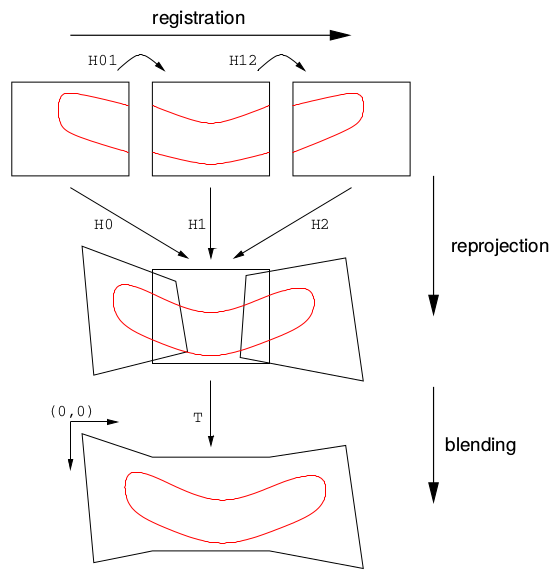
\includegraphics[width=10cm]{registration-process}}
	\caption{Proceso básico para la generación de mosaico, poner referencia, cambiar a español}
	\label{imagen:mosaic-process}
\end{figure}

Si bien, se han propuesto una gran cantidad de algoritmos por parte de distintos grupos de investigación en todo el mundo, esta tarea aun sigue siendo desafiante, debido mayormente a los procesos de registro y fusión de las imágenes. Específicamente el proceso para estimar correspondencias entre las imágenes es un problema complicado, en principio debido a la naturaleza no plana de los suelos estudiados; por otro lado la reducción de discontinuidades, o inconsistencias entre imágenes consecutivas sigue siendo una tarea desafiante. De modo que la mayoría de avances e implementaciones en esta área están encaminados en resolver estos dos problemas principales, o bien mejorar los resultados de trabajos previos. De esta forma se clasificarán los algoritmos para la generación de mosaicos basados en como estos abordan los procesos de registro y fusión, además para cada clasificación se realiza una revisión teórica de cada categoría, así como también los diferentes métodos y modificaciones que han aplicado los distintos desarrolladores. 

\subsection*{Clasificación basada en el registro de imágenes}

Este proceso es muy importante para la creación de mosaicos, y básicamente es la base para estos. Cuando se registran imágenes, primero lo que se busca es encontrar la relación, o la correspondencia entre estas. donde estas pudieron haber sido capturadas desde distintos puntos de vista, distintos instantes de tiempo, distinta perspectiva, o incluso distintas cámaras. Luego de encontrar las zonas o puntos correspondientes se busca estimar una matriz de transformación geométrica que permita alinearlas todas en los pasos siguientes. Se puede decir que el registro ha sido exitoso, si se logra estimar una matriz de transformación tal que todos los puntos correspondientes se puedan unir.

Las relaciones entre las imágenes se pueden establecer utilizando distintos métodos, ya sea, emparejando puntos coincidentes, regiones enteras, o bien usando la propiedad de correlación de fase en el dominio de la frecuencia. Estos métodos para establecer correspondencias son discutidos a continuación.

\subsubsection*{Algoritmos en el dominio espacial}

Los algoritmos en esta categoría utilizan la información de los píxeles para establecer la relación entre imágenes, es decir, se utiliza el valor de los píxeles (intensidad) y se trata de establecer la correspondencia de estos según la ubicación en la que se encuentren. Estos se pueden separar en dos técnicas principales: basados en área o en puntos clave.

Los algoritmos basados en área, buscan relacionar dos ventanas o regiones en dos imágenes que correspondan a la misma escena. El concepto principal consiste en mover la región de interés desde la primera imagen hacia la segunda, buscando que la diferencia entre las intensidades sea la menor posible, es decir,  se trata de estimar la mejor matriz de transformación que logre reducir la diferencia de intensidades al alinear las regiones estudiadas (citar). Algunos trabajos importantes en esta clasificación utilizaron algoritmos como NCC (citar), y el MI (citar), donde estos proporcionan una métrica de similitud entre dos imágenes. Al emplear esta técnica se logra emparejar las imágenes a nivel de píxel, si bien se logran buenos resultados, el proceso de iterar para optimizar los parámetros de transformación y el calculo del error para cada píxel sobre las regiones, se convierte computacionalmente costoso.

Para reducir el tiempo de computo, se utilizan algoritmos basados en características, en los cuales se tratan de detectar puntos en distintas imágenes, que correspondan con el mismo. De este modo se puede encontrar la transformación geométrica que relaciona estos puntos de origen con los de destino resolviendo una ecuación lineal.


\subsection*{Clasificación basada en el fusión de imágenes}


\section{Esquema propuesto}

\begin{figure}[H]
	\centerline{
		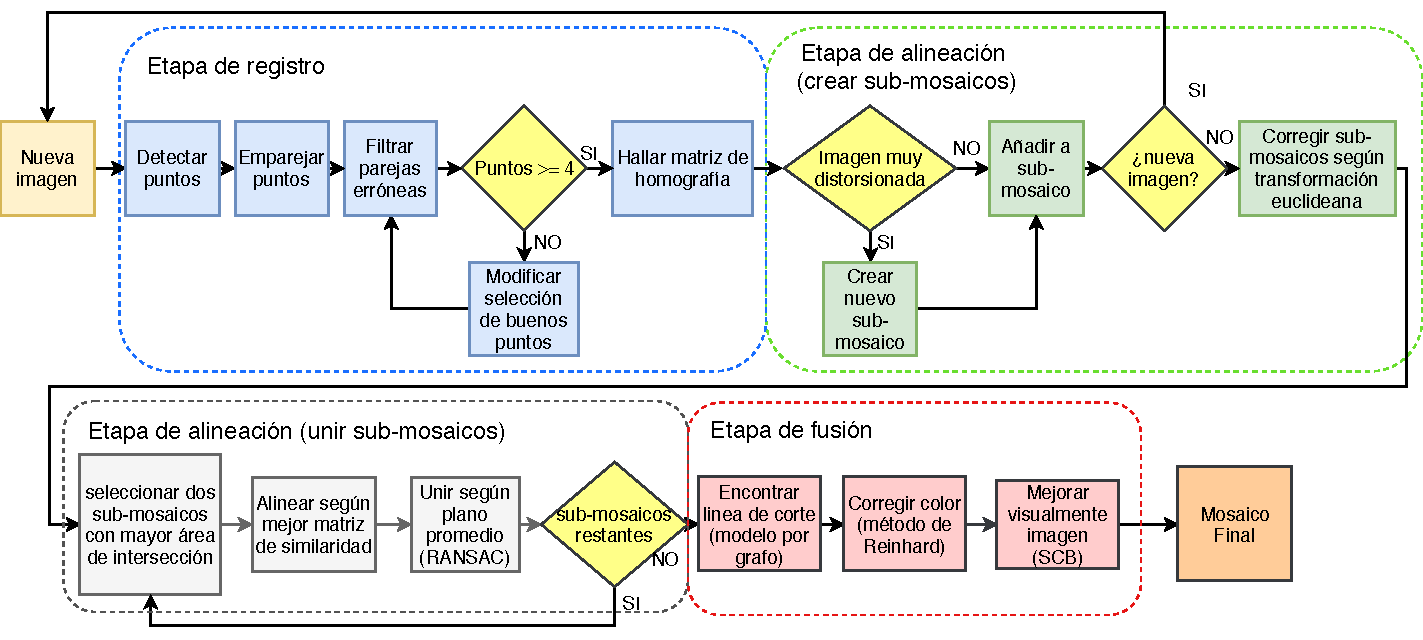
\includegraphics[width=1.21\textwidth]{esquema-general}}
		\caption{Esquema propuesto para la construcción del mosaico}
	
	\label{imagen:esquema}
\end{figure}

\section{OpenCV}